

\documentclass{article}

\usepackage{graphicx}
\usepackage[margin=0.6in]{geometry}
\usepackage{mathtools}
\usepackage{amssymb}
\usepackage{fancyvrb}
\usepackage[parfill]{parskip}
\DefineVerbatimEnvironment{code}{Verbatim}{fontsize=\small}
\DefineVerbatimEnvironment{example}{Verbatim}{fontsize=\small}
\usepackage[framed]{mcode}




\begin{document}

\begin{titlepage}
\thispagestyle{empty}
\title{B1 Engineering Computation Project \\ Wireless Communication Channels: \\
Characterisation using orthogonal functions}
\author{James Routley \\
    Trinity College, Oxford \\
    6th January 2013 \\
    \texttt{james.routley@trinity.ox.ac.uk}}
\date{\today}
\maketitle    

\end{titlepage}














\section*{Introduction}

The aim of this project is to investigate the statistical properties of Wifi systems operating indoors. We shall do this by using a set of orthogonal basis functions called \emph{Laguerre functions} to construct a mathematical model of the probability density function describing the attenuation caused by the scattering process in the wireless communication medium. 

The project starts by showing how orthogonality is a useful property. We go on to investigate Gram-Schmitt Orthogonalisation before generating and using Laguerre functions to model the wifi data given to us. 
















\section{Orthogonality}

We can use orthogonal basis functions to model our data. Orthogonality is desirable because we can add more terms without changing the values of previously calculated coefficients. Orthogonal basis functions take the form:

$${f(0) = a_0g_0(x) + a_1g_1(x) + a_2g_2(x) + a_3g_3(x) + ... }$$
















\section{Fourier Series}

A common orthogonal basis is set the Fourier series. The functions $cos(n \omega x)$ and $sin(n \omega x)$, for  $n = 0, 1, ... $  form an orthogonal set when the inner product is defined by the integral over a period ${T = \frac{2\pi}{\omega}}$, divided by the period.















\subsection{Using Matlab to compute Fourier series}

\subsubsection{Testing Orthogonality}

We are given a function \mcode{fs_orthog.m} which integrates Fourier basis functions over a period. We are asked to write some code, \mcode{fs_orthogtest.m}, which calls this function for $cos(m x) \times cos(n x)$ for ${m = 0 \to 6}$ and ${n = 0 \to 6}$ and stores the result in a 2D matrix:

\begin{lstlisting}
coscos = zeros(7); %set up a 7x7 matrix of zeroes to store the integral results

for m = 0 : 6
    for n = 0 : 6
        coscos(m+1, n+1) = fs_orthog(1, 1000, m, n, 'cc'); 
    end
end
\end{lstlisting}


We later repeat this code to include $sin(m x) \times sin(n x)$ and $cos(m x) \times sin(n x)$

%{What is the reason for this failure?}













\subsubsection{Code to Compute Fourier Series Coefficients}

To compute the Fourier series coefficients, we are given two pieces of code, \mcode{fs_Acoeff.m} and \mcode{fs_Bcoeff.m} which calculate the $ A_m $ and $ B_m $ coefficients respectively. These functions are called from a top level script, \mcode{fs_triangle.m} to plot a graph of the Fourier series approximation of a periodic function. The periodic function, a triangle wave:


$$
	f(x)=\begin{cases}
	1+2x  &\text{ for } -\frac{1}{2}<  x< 0 \\ 
	1-2x  &\text{ for }  \:\:\:\:\:\:0<  x< \frac{1}{2}  
	\end{cases}
$$



is generated by \mcode{fs_periodictriangle.m}.

We create a function which generates a Fourier approximation to the triangle wave given $n$, the number of Fourier terms we are interested in. The Fourier approximation with four terms is shown in Figure \ref{fourierapproximationtriangle}. 




\begin{figure}[h]
\centering
	\begin{minipage}[c][][b]{0.45\linewidth}
		\begin{center}
		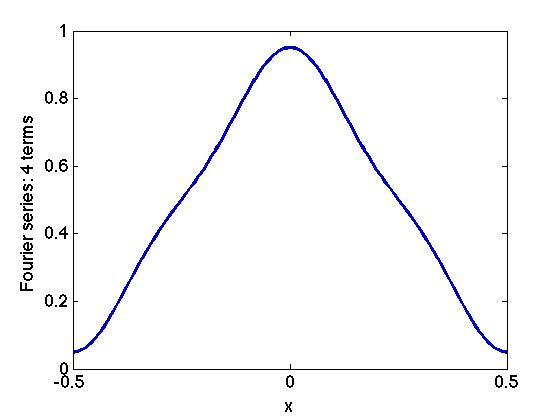
\includegraphics[scale=0.35]{Matlab/Fourier/Images/fs_triangle4.jpg}  
		\end{center}
		\caption[b]{Fourier approximation of a triangle with $n = 4$}
		\label{fourierapproximationtriangle}
	\end{minipage}
\quad\quad\quad\quad
	\begin{minipage}[c][][b]{0.45\linewidth}
		\begin{center}
		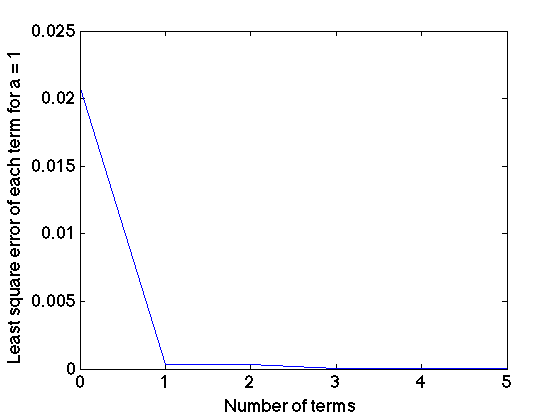
\includegraphics[scale=0.35]{Matlab/Fourier/Images/errorAEquals1.png}
		\end{center}
		\caption[b]{Number of terms in a Fourier approximation to a triangle function against the error of the approximation}
		\label{numberoffourierterms}
	\end{minipage}
\end{figure}



To judge the quality of the Fourier approximation as the number of $ n-terms $ changes, the function \mcode{fs_triangleerror.m} compares the least square error between the Fourier approximation and the actual triangle as the number of $ n-terms $ varies. The results are shown in Figure \ref{numberoffourierterms}

I created a new function \mcode{fs_periodictrianglenew.m} which generates the periodic function in Figure \ref{periodtrinew}.



\begin{figure}[h]
\centering
	\begin{minipage}[c][][b]{0.45\linewidth}
		\begin{center}
		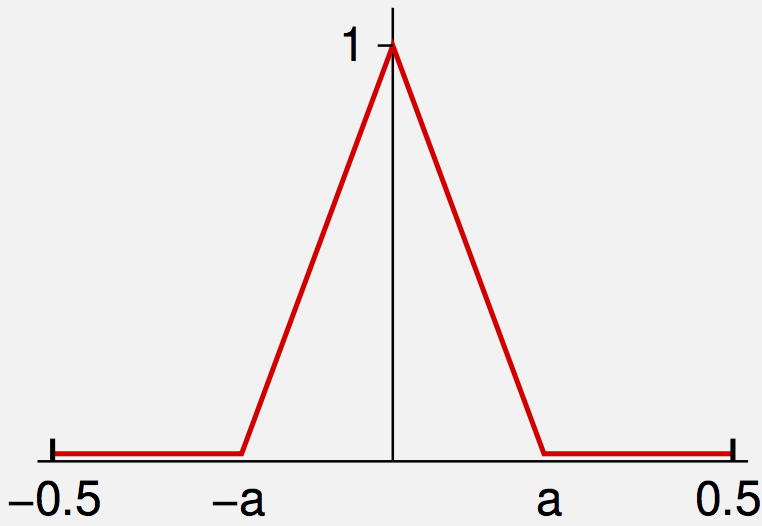
\includegraphics[scale=0.25]{Matlab/Fourier/Images/fs_periodictrianglenew.png}  
		\end{center}
		\caption[b]{The function generated by \mcode{fs_periodictrianglenew}}
		\label{periodtrinew}
	\end{minipage}
\quad\quad\quad\quad
%	\begin{minipage}[c][][b]{0.45\linewidth}
%		\begin{center}
%		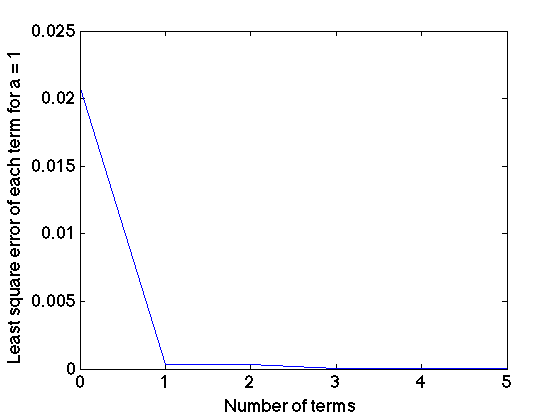
\includegraphics[scale=0.35]{Matlab/Fourier/Images/errorAEquals1.png}
%		\end{center}
%		\caption[b]{REPLACE}
%		\label{}
%	\end{minipage}

\end{figure}

Fourier approximations model functions using $sin$ and $cos$ curves. This means that the more unlike a $sin$ or $cos$ curve the function is, the more terms will be needed to generate a good model. As $a$ decreases, the more unlike a $cos$ curve it becomes, therefore requiring more terms. 

The $B_m$ terms refer to the $sin$ terms in the Fourier approximation are always around $0$. This is because the function that we are modelling is even, and so the Fourier approximation will only be made up of even $cos$ terms.  



















\section{The Gram-Schmidt Process}



The Gram-Schmidt process is a method of orthogonalising a set of linearly independent functions. To do so, we take the 0th function and orthogonalise the rest of the functions in relation to it. We subtract a projection of the 0th function onto the 1st function from the 1st function. We repeat this with the 2nd function, subtracting projections of the 0th and the 1st functions from it, and so on. This can be represented mathematically:
$$
\begin{aligned}
g_0(x) &= v_0(x) \\
g_1(x) &= v_1(x) -e\_{10}g_0(x) \\
g_2(x) &= v_2(x) -e\_{20}g_0(x) -e_{21}g_1(x) \\
\end{aligned} \\
$$

This gives us an orthogonal basis set of functions $ g_0(x),\ g_1(x),\ g_2(x),\ ...$.

The $e$ values are the coefficients representing the projections of function onto each other. They can be calculated:

$$ e_{10} =  \frac{\langle v_1, g_0 \rangle}{\langle g_0, g_0 \rangle} $$

















\subsection{Using Gram-Schmitt Orthogonalisation}

We are to perform Gram\textunderscore Schmitt orthogonalisation on the linearly independent set of monomials:

$$
\begin{aligned}
v_0(x) &= 1 \\
v_1(x) &= x \\
v_2(x) &= x^2 \\
\ldots
\end{aligned} \\
$$


with respect to the inner product:

$$ 
\langle g_n, g_m \rangle = \int_0^\infty \ g_n(x)g_m(x)e^{-x} \, \mathrm{d}x 
$$

My code is run by calling a top level script, \mcode{gs_script.m}. The parameters of how many monomials to linearise and the range of x values to look at are defined within the script. The script calls on a series of functions to complete small tasks:

\begin{enumerate}
  \item Generate a matrix, $G$, of the monomials.
  \item Perform Gram-Schmitt orthogonalisation upon the matrix G to produce a matrix of orthogonal functions, $V$ and a matrix of coefficients, $E$.
  \item Normalise $V$ and verify orthonormality of $\tilde{V}$
  \item Plot the orthonormal functions $\tilde{v_0},\ \tilde{v_1},\ \tilde{v_2},\ ...   $
\end{enumerate}

The Gram-Schmitt orthogonalisation is performed by a function \mcode{gs_gramschmittorthogonalisation.m}:


\begin{lstlisting}

function [E, G] = gs_gramschmittorthogonalisation(V, n, x)

    E = zeros(n, n-1);			%create empty matrices E and G
    G = zeros(n, length(x));
    G(1, :) = V(1, :);			%Set g0 = v0

    for k = 1 : n-1
        G(k+1, :) = V(k+1, :);	%set gk = vk
        for l = 1 : k
            %calculate e and store it in E
            E(k+1, l) = gs_innerproduct(x, V(k+1, :), G(l, :)) / gs_innerproduct(x, G(l, :), G(l, :));
            %subtract the projection of previous functions from the function in question 
            G(k+1, :) = G(k+1, :) -  E(k+1, l) .* G(l, :);
        end
    end
end


\end{lstlisting}

The nested for loops cycle through the rows of the $V$ vector, calculating $e$ values before subtracting the projection of the previous functions from the one in question.  


The inner product is calculated in \mcode{gs_innerproduct.m} using Matlab's trapz function:

\begin{lstlisting}
function [result] = gs_innerproduct(x, y1, y2)
    result = trapz(x, y1.*y2.*exp(-x));
end
\end{lstlisting}

Figure \ref{gsorthogonalisation} shows the normalised Gram-Schmitt vectors. Figure \ref{evalues} shows the $e$ coefficients, which have been converted to integers using MATLAB's int16() function. 

\begin{figure}[h]
\centering
	\begin{minipage}[c][][b]{0.45\linewidth}
		\begin{center}
		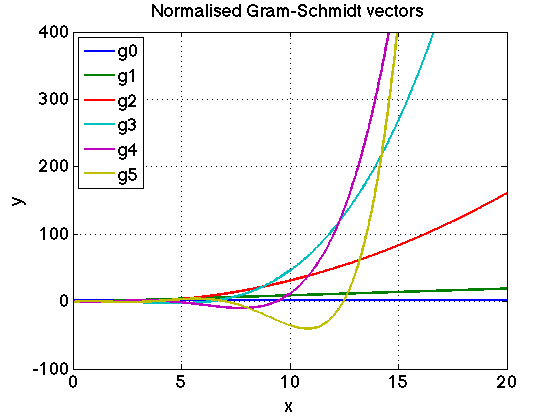
\includegraphics[scale=0.35]{Matlab/GramSchmidt/Images/gsorthogonalisation.png}  
		\end{center}
		\caption[b]{Normalised Gram-Schmitt Vectors}
		\label{gsorthogonalisation}
	\end{minipage}
\quad\quad\quad\quad
	\begin{minipage}[c][][b]{0.45\linewidth}
		\begin{center}
		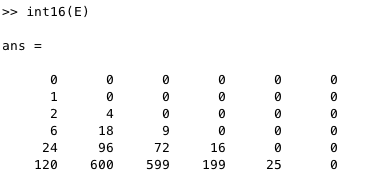
\includegraphics[scale=0.6]{Matlab/GramSchmidt/Images/gs_Evalues.png}
		\end{center}
		\caption[b]{$e$ coefficients}
		\label{evalues}
	\end{minipage}

\end{figure}


%4. describe the computational experiments you designed and performed to verify its performance,
%5. give results, and importantly,
%6. draw conclusions.






















\section{Laguerre} 
\subsection{Laguerre Polynomials}

Laguerre polynomials are a set of polynomials which are orthogonal with respect to the exponential weighting function. They can be generated using the \emph{Rodrigues formula}:

$$
L_n^{(\alpha)}(x) = \frac{1}{n!} x^{-\alpha} e^x \frac{d^n}{dx^n}(x^{n+\alpha} e^{-x}),\    n \in  \mathbb{N}, \alpha \in \mathbb{R} 
$$


We can see that for the $n^{th}$ derivative, the $x^{a}e^{-x}$ can be factored out and cancels with the $x^{-a}e^{x}$. This means we only need to find the coefficients of the polynomial and multiply them by $\frac{1}{n!}$

















\subsection{Calculating Coefficients of the $n^{th}$ Laguerre Polynomial}

These polynomial coefficients are calculated in Matlab using the function \mcode{l_laguerrecoefficients.m}

\begin{lstlisting}
function c = l_laguerrecoefficients(n, a)
    
    c = 1/factorial(n) .* binomials(n) .* fcoeff(n, a) .* gcoeff(n);
    
end
\end{lstlisting}

Running the code for $ n = 5 $ and $ \alpha = 1 $ produces the results $-0.0083,\  0.2500,\  -2.5000\  10.0000\  -15.0000\  6.0000$ as expected. 



















\subsection{Calculating Laguerre Polynomials Recursively}

We then write code which successively computes the Laguerre polynomials up to order $ n $.

Our top level script, \mcode{l_recurrsivelaguerre.m} calls upon the function \mcode{l_recurrsivelaguerrecoefficients.m} to generate a matrix of Laguerre coefficients.  

\begin{lstlisting}

function C = l_recurrsivelaguerrecoefficients(n, a)

%set up matrix C
    C = zeros(n);
    C(1, n) = 1;
    C(2, n-1 : n) = [-1, a + 1];

%cycle through rows and calculate and store coefficients
    for i = 3:n
        
%caclculate the values of the coefficients of the recurring section of
%equation
        reccoeff1 = [-1 , (2*(i-1) + a -1)];
        reccoeff2 = ((i-1) + a -1);
        
%multiply the polynomials together using conv
        x = conv(reccoeff1, C(i-1, :));
        x(1) = [];          %corrects for syntax error caused by using conv
        y = conv(reccoeff2, C(i-2, :));
        
%subtract one polynomial from the other and store in C
        C(i, :) = 1/(i-1)*(x - y);
    end
end
\end{lstlisting}

The code uses the MATLAB function conv to do the necessary multiplication of two polynomials. 

The script then generates generates a matrix of values representing the equations:

$$
\begin{aligned}
y &= 1 \\
y &= x \\
y &= x^2 \\
&\vdots \\
y &= x^n
\end{aligned} \\
$$

and multiplies the relevant equations with the relevant coefficients to generate the Laguerre Polynomials or order up to $ n $.

The Laguerre polynomials for $n = 5$ and $\alpha = 0$ are shown in Figure \ref{recursivepolynomials}
















\subsection{Comparison of Laguerre and Gram-Schmitt Polynomials}

It is noticed that the definition of the inner product for the Gram-Schmitt Process is identical to that for the Laguerre polynomials, when $\alpha = 0$. 

To investigate this, we plot the difference between the Gram-Schmitt Orthogonalised polynomials $\tilde{G}_n^{(x)} $ and the Laguerre polynomials when $\alpha = 0$, using the function \mcode{l_compareGandL}. 

The results are shown in Figure \ref{G-Lbefore}, and show that Gram-Schmitt - Laguerre is roughly $0$ for even terms but are not $0$ for odd terms. To correct for this, we change the monomials $v_n$ upon which we perform Gram-Schmitt Orthogonalisation from $v_n = x^n$ to $v_n = (-x)^n$. 

\begin{figure}[h]
\centering
	\begin{minipage}[c][][b]{0.45\linewidth}
		\begin{center}
		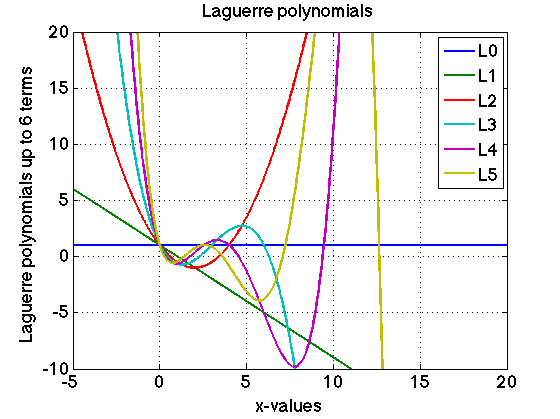
\includegraphics[scale=0.35]{Matlab/Laguerre/Graphs/RecursivePolynomials.png}
		\end{center}
		\caption[b]{Laguerre polynomials for $n = 5$, $\alpha = 2$}
		\label{recursivepolynomials}
	\end{minipage}
\quad\quad\quad\quad
	\begin{minipage}[c][][b]{0.45\linewidth}
		\begin{center}
		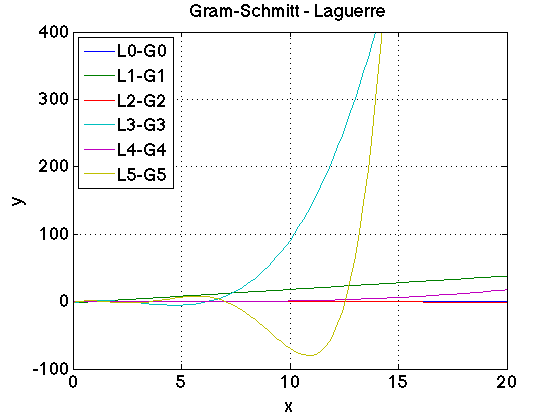
\includegraphics[scale=0.35]{Matlab/Laguerre/Graphs/G-Lbefore.png}  
		\end{center}
		\caption[b]{Gram-Schmitt - Laguerre}
		\label{G-Lbefore}
	\end{minipage}

\end{figure}



















\subsection{Associated Laguerre Polynomials}

We write code which produces a set of associated Laguerre functions, an orthonormal subset of the Laguerre polynomials:
$$
\psi_n^{(\alpha)} (x) = \sqrt{\dfrac{\Gamma(n+1)}{\Gamma(n+\alpha+1)}} x^{\alpha/2} e^{-x/2} L_n^{(\alpha)}
$$

To do this we make use of MATLAB's gamma() function. The function \mcode{l_generateL} called generates the Laguerre polynomial $ L_n^{(\alpha)} $.

\begin{lstlisting}
function psi = l_generatepsi(x, n, a)

    L = l_generateL(x, n, a);
    psi = sqrt((gamma(n+1))/gamma(n+a+1)).*L(n,:).*x.^(a/2).*exp(-x/2);
end
\end{lstlisting}

A function \mcode{l_plotpsi} is used to plot $\psi_0^{(\alpha)}, \psi_1^{(\alpha)}, ...,  \psi_5^{(\alpha)} $ in the range $ 0 \le x \le 40 $ for $ \alpha = 0,2 $ (Figures \ref{psi0} and \ref{psi2})


\begin{figure}[h]
\centering
	\begin{minipage}[c][][b]{0.45\linewidth}
		\begin{center}
		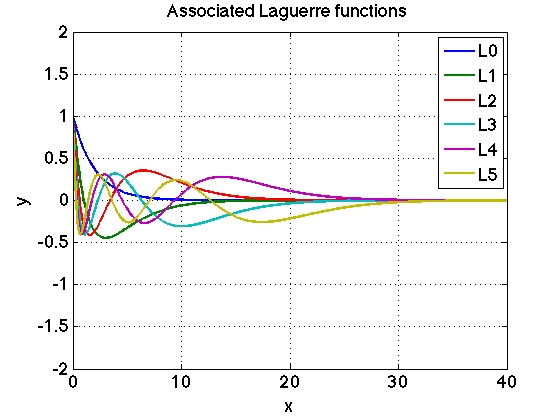
\includegraphics[scale=0.35]{Matlab/Laguerre/Graphs/psi0.png}  
		\end{center}
		\caption[b]{Associated Laguerre Polynomials up to $n = 5$, where $\alpha = 0$}
		\label{psi0}
	\end{minipage}
\quad\quad\quad\quad
	\begin{minipage}[c][][b]{0.45\linewidth}
		\begin{center}
		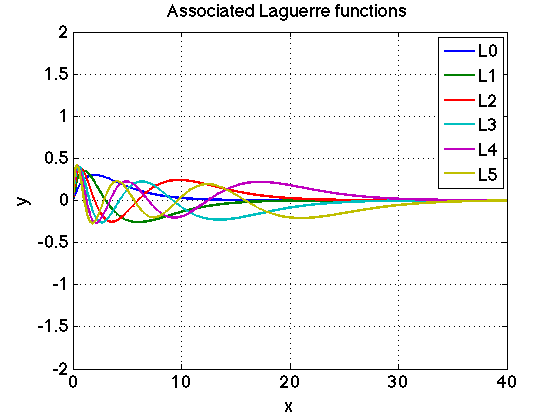
\includegraphics[scale=0.35]{Matlab/Laguerre/Graphs/psi2.png}
		\end{center}
		\caption[b]{Associated Laguerre Polynomials up to $n = 5$, where $\alpha = 2$}
		\label{psi2}
	\end{minipage}

\end{figure}












\section{Fitting to Synthesised Data}

We model our data by equating it to a series of ortogonal associated Lageurre functions, $\psi_n$ (which we have previously generated), multiplied by their respective coefficients, $\alpha_n$:

$$
f(x) = a_0\psi_0(x) + a_1\psi_1(x) + a_2\psi_2(x)\ldots\\
$$

The coeffificients can be worked out using the inner product:

$$
a_n = \langle \psi_n,f_o\rangle/\langle \psi_n,\psi_m\rangle = \int_{0}^{\infty} \psi_n(x)f_o(x)dx 
$$



We are given a function, \mcode{exp_data} which generates the density function associated with a set of exponentially distributed data. This function has four inputs, \mcode{sigma2, mu, nsamp, nbins}, which refer to; variance, mean, number of samples and the number of data points generated respectively. 



% Run the code for different input values to explore how it works. Include any noteworthy observations in your report. 



















\subsection{Laguerre Fitting Function}

We create a function \mcode{fd_laguerrefit} which implements the above mathematics to generate a Leguerre fit to the data supplied by \mcode{exp_data}, using the associated Laguerre functions. 

\begin{lstlisting}
function [f] = fd_laguerrefit(n,a,fo,x)
% generate psi vectors
psi = fd_generatepsi(x, n, a);      

% set up empty vector for alpha coefficients
a_n = zeros(1,n);

% generate alpha coefficients
for i = 1:n;
    func = psi(i,:).*fo;
    a_n(1,i) = trapz(x,func);
end

% add together terms in Laguerre fitting
 f = a_n(1,1).*psi(1,:);
 for i = 2:n;
     f = f + a_n(1,i)*psi(i,:);
 end
\end{lstlisting}


%Run the code in Code Box A below. What does the data in fo look like? Is it decaying/increasing? How quickly (describe qualitatively)?

Figure \ref{lfitdata} shows the data generated by \mcode{exp_data}, when imput with \mcode{ sigma2 = 2; mu = 0; nsamp = 1e4 ; nbins = 100;}. This data is decaying exponentially. %DESCRIBE DATA

\begin{figure}[h]
\centering
	\begin{minipage}[c][][b]{0.45\linewidth}
		\begin{center}
		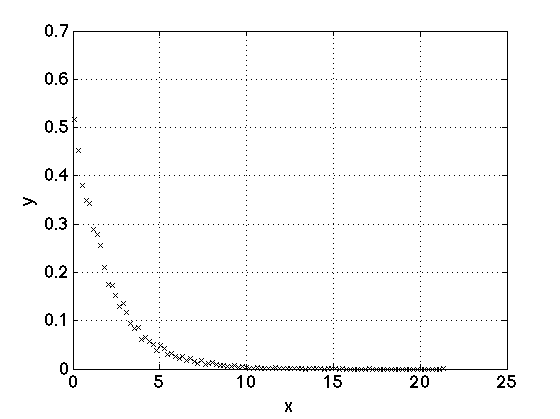
\includegraphics[scale=0.35]{Matlab/FittingData/Graph/lfitdata.png}  
		\end{center}
		\caption[b]{Data generated by the \mcode{exp_data} function}
		\label{lfitdata}
	\end{minipage}
\quad\quad\quad\quad
	\begin{minipage}[c][][b]{0.45\linewidth}
		\begin{center}
		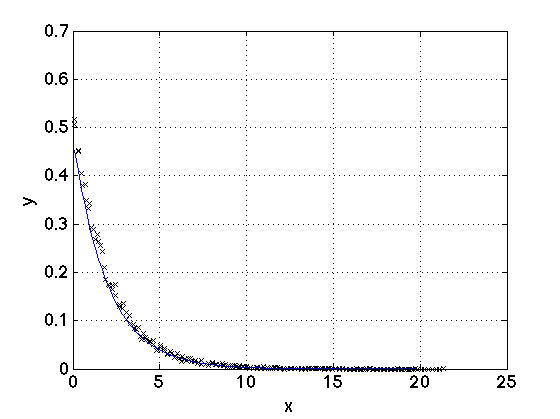
\includegraphics[scale=0.35]{Matlab/FittingData/Graph/Lfitn0.png}
		\end{center}
		\caption[b]{The $0^{th}$ order Laguerre fit to the data previously produced.}
		\label{lfit0}
	\end{minipage}

\end{figure}

















\subsection{Laguerre Fit}

We generate the $0^{th}$ order Laguerre fit to the data previously produced (Figure \ref{lfit0}). 

We find that $a_0 = 0.4774$ %is this what we expected? Write the equation for this fit

\subsection{Parameterised Fit}

When \mcode{sigma2 = 2 and mu = 0}, the function \mcode{exp_data.m} generates an exponentially distributed random variable with an expected value of 2. We expect a fit of $f(x) = \frac{1}{2} e^{-\frac{x}{2}}$. A basic parameterised fit can be made using the mean of the data $\xi$:

$$
f(x) = \frac{1}{\xi}e^{-\frac{x}{\xi}}
$$

The mean, $\xi$, and the parameterised fit are calculated with the code:

\begin{lstlisting}
estimated_mean = trapz (x , x .* fo )
p_fit = 1/estimated_mean.*exp(-x/estimated_mean);
\end{lstlisting}




We use this parameterised fit as a comparison to the Laguerre fits that we generate. 

We then compare the accuracy of the Parameterised fit with the $0^{th}$ order Laguerre fit (Figure \ref{compareLandP}) by comparing the errors of each fit using \mcode{fd_script1}:

$$
error = \int_{0}^{\infty }(f(x)-f_0(x))^2
$$

We find that the Laguerre Error $= 0.003762$ while the Parameterised Error $= 0.001589$. 

\begin{figure}[h]
\centering
	\begin{minipage}[c][][b]{0.45\linewidth}
		\begin{center}
		\includegraphics[scale=0.35]{Matlab/FittingData/Graph/compareLandP.png}  
		\end{center}
		\caption[b]{A comparison of the Laguerre fit and the parameterised fit to the data}
		\label{compareLandP}
	\end{minipage}
\quad\quad\quad\quad
%	\begin{minipage}[c][][b]{0.45\linewidth}
%		\begin{center}
%		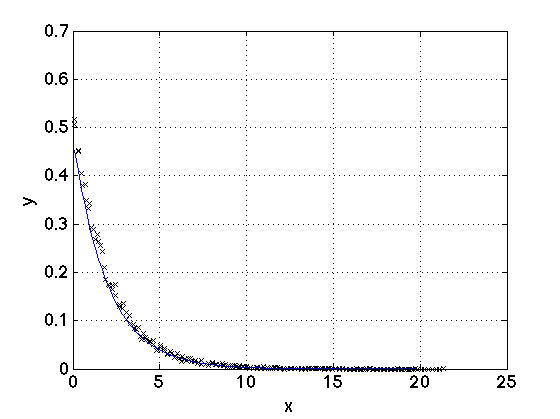
\includegraphics[scale=0.35]{Matlab/FittingData/Graph/Lfitn0.png}
%		\end{center}
%		\caption[b]{REPLACE}
%		\label{}
%	\end{minipage}

\end{figure}













\subsection{Varying $\alpha$}

In the previous example, the Laguerre function with $\alpha = 0$ fitted the data well, but this will not always be the case. We can vary this parameter in order to provide a better fit. 

To demonstrate this, we generate Laguerre fits, up to the $5^{th}$ order, for $\alpha = 0, 2$ and calculate the error associated with the fit. (Figures \ref{dataa0} and \ref{dataa2})


\begin{figure}[h]
\centering
	\begin{minipage}[c][][b]{0.45\linewidth}
		\begin{center}
		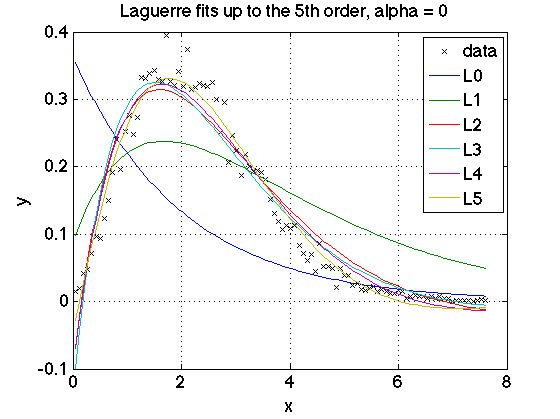
\includegraphics[scale=0.35]{Matlab/FittingData/Graph/fitdataa0.png}  
		\end{center}
		\caption[b]{Laguerre fits to to the $5^{th}$ order, where $\alpha = 0$}
		\label{dataa0}
	\end{minipage}
\quad\quad\quad\quad
	\begin{minipage}[c][][b]{0.45\linewidth}
		\begin{center}
		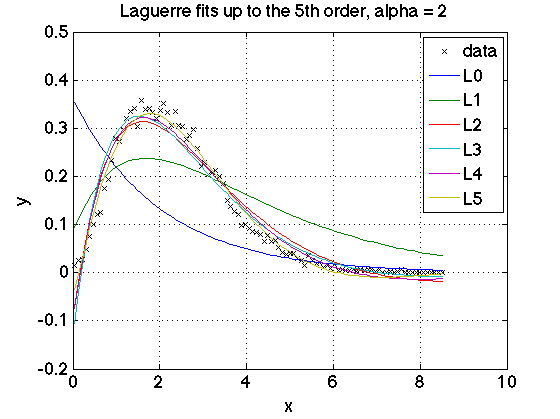
\includegraphics[scale=0.35]{Matlab/FittingData/Graph/fitdataa2.png}
		\end{center}
		\caption[b]{Laguerre fits to to the $5^{th}$ order, where $\alpha = 2$}
		\label{dataa2}
	\end{minipage}
\end{figure}

The parameterised errors for $\alpha = 0$ are consistently lower: 
\begin{lstlisting}
%Laguerre Error for alpha=0:
   0.1143   0.04081   0.006485   0.006125   0.004647   0.002373

%Laguerre Error for alpha=2:
   0.04427   0.01092   0.01102   0.006551   0.002694   0.001231
\end{lstlisting}

%WHY? CAN WE PREDICT? 










\subsection{Scaling and Offsetting}



Laguerre polynomials are canonical, and so if we wish to use them to model data which does not pass though the origin, we must scale the x values used, such that $xscaled = \frac{x - \xi}{\sigma}$. In the code this is achieved by using \mcode{xscaled = 2* x / sigma2;}. The factor of $2$ originates from or defining of $var = sigma2 = 2\sigma $. 

We generate a Laguerre fit to some data provided (Figure \ref{part3,1}). It is shown that all of the unscaled Laguerre fits pass through $(0,0)$. As the data provided passes through $(0,0.2)$, there is a limit to the accuracy that we will be able to achieve. As the number of $n-terms$ increases, the polynomials are able to correct for this more but still miss the points closest to $x=0$. The scaled results are shown in Figure \ref{part3,2}.
%Plot your results. Are any of these fits suitable? Deduce whether or not you would be able to obtain a `good' fit for this data by using some arbitrary order of expansion; explain your reasoning. (Hint: Pay particular attention to the origin.)

\begin{figure}[h]
\centering
	\begin{minipage}[c][][b]{0.45\linewidth}
		\begin{center}
		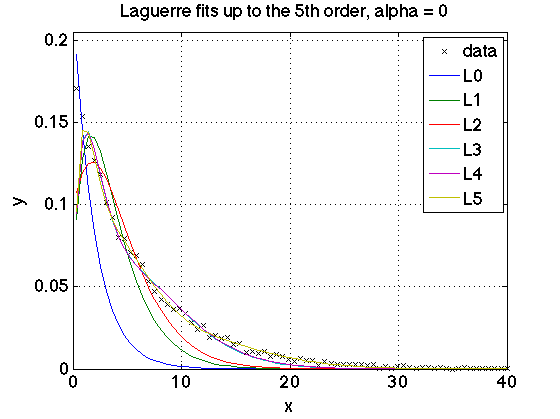
\includegraphics[scale=0.35]{Matlab/FittingData/Graph/part3,1.png}  
		\end{center}
		\caption[b]{Laguerre fits to to the $5^{th}$ order, where $\alpha = 0$}
		\label{part3,1}
	\end{minipage}
\quad\quad\quad\quad
	\begin{minipage}[c][][b]{0.45\linewidth}
		\begin{center}
		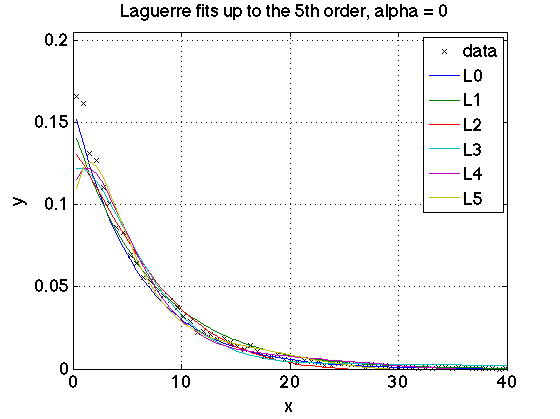
\includegraphics[scale=0.35]{Matlab/FittingData/Graph/part3,2.png}
		\end{center}
		\caption[b]{Laguerre fits to to the $5^{th}$ order, where $\alpha = 2$}
		\label{part3,2}
	\end{minipage}

\end{figure}


By scaling the $x values$ that we use, we can correct for this error. As shown, the scaled results  are more accurate, but that accuracy decreases as the order increases for the scaled. 

\begin{lstlisting}
Unscaled Laguerre Error =

   0.02443   0.006570   0.004345   0.002169   0.002164   0.001799

Scaled Laguerre Error =

   1.0e-03 *
   0.3010   0.4890   0.6138   0.6975   0.7501   0.7709
   
Parameteric Error =

   7.805763883796818e-04
   
\end{lstlisting}


%include graph part3,3.png

%Write down the equation for the new 0th order fit. How does this compare to a parameterised fit vis-a-vis Eq. (5.13)?








\section{Fitting to a Real Data Set}

We try to find a model for the observed wifi data, stored in \mcode{measured_data.mat}. The function \mcode{fd_fit_measured_data.m} runs the code generating a scaled Laguerre fit to the data, for a given $n$ $\alpha$, outputting the error value of the approximation. 

Our data does not pass though the origin (Figure \ref{dataorigin}), and is not an exponential decay (Figure \ref{laguerrefit62}) and so the standard Laguerre fit and the Parameteric fits are not appropriate. We will therefore use a scaled Laguerre fit to model the wifi data. 

\begin{figure}[h]
\centering
	\begin{minipage}[c][][b]{0.45\linewidth}
		\begin{center}
		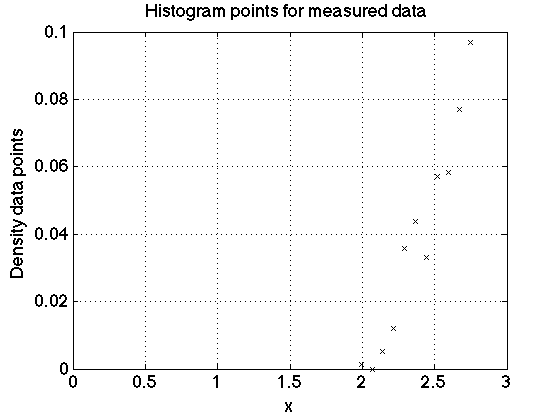
\includegraphics[scale=0.35]{Matlab/FittingData/Graph/dataorigin.png}  
		\end{center}
		\caption[b]{The provided data does not pass through the origin}
		\label{dataorigin}
	\end{minipage}
\quad\quad\quad\quad
	\begin{minipage}[c][][b]{0.45\linewidth}
		\begin{center}
		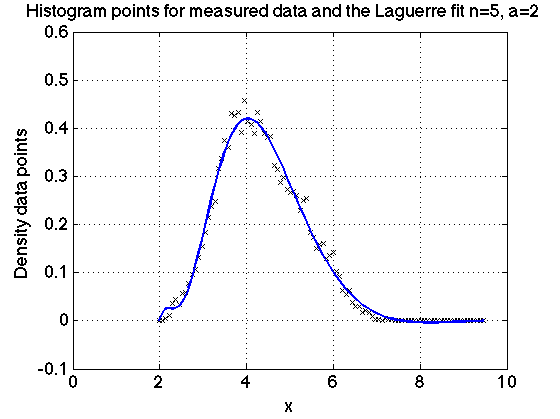
\includegraphics[scale=0.35]{Matlab/FittingData/Graph/laguerrefit62.png}
		\end{center}
		\caption[b]{Data provided and the scaled Laguerre fit where $n=5$ and $\alpha = 2$}
		\label{laguerrefit62}
	\end{minipage}

\end{figure}

The script \mcode{fd_testmeasureddatascript.m} uses two nested for loops to cycle though all combination of $n$ and $\alpha$, storing the error values in a matrix E. \mcode{fd_plotE} plots the error values against $\alpha$ values for the different orders of Laguerre fit (Figures \ref{EvsAbig} and \ref{EvsAsmall}). 

\begin{figure}[h]
\centering
	\begin{minipage}[c][][b]{0.45\linewidth}
		\begin{center}
		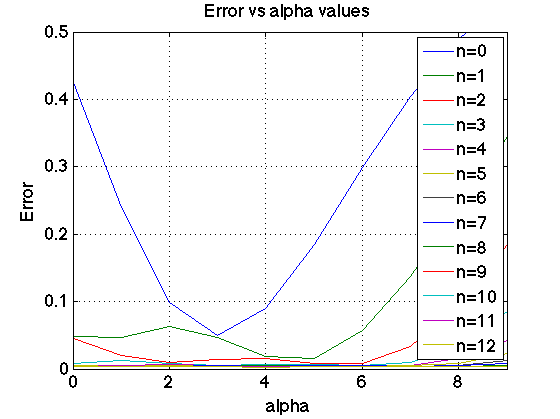
\includegraphics[scale=0.35]{Matlab/FittingData/Graph/EvsAbig.png}  
		\end{center}
		\caption[b]{Error values vs $\alpha$ values for a range of $n$ values}
		\label{EvsAbig}
	\end{minipage}
\quad\quad\quad\quad
	\begin{minipage}[c][][b]{0.45\linewidth}
		\begin{center}
		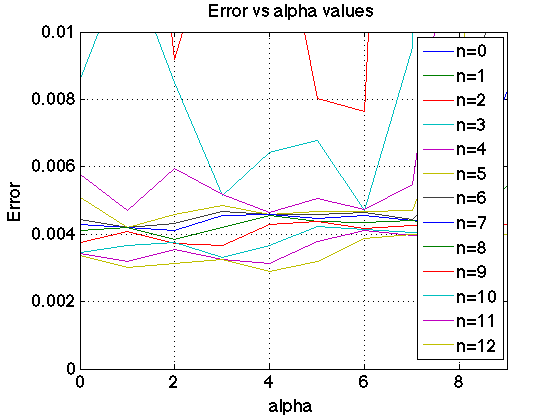
\includegraphics[scale=0.35]{Matlab/FittingData/Graph/EvsAsmall.png}
		\end{center}
		\caption[b]{Error values vs $\alpha$ values for a range of $n$ values (zoomed in)}
		\label{EvsAsmall}
	\end{minipage}

\end{figure}

As we can see from the graphs, the errors level out after $n=5$, and so for the sake of the speed of the code, I will look a Laguerre fit of the $5^{th}$ order, even though a more accurate result could be found by using a higher order. With high order polynomials, small changes to coefficients can result in large changes to the function produced, amplifying errors. For $n=5$, the best result is with $\alpha = 2$, giving an error of $0.004195$. The Laguerre fit for these values are plotted in Figure \ref{laguerrefit62}





\section{Conclusion}


In this project we have investigated using orthogonal functions to model data. We started by investigating Fourier approximations which use the orthogonality of $sin$ and $cos$ functions. We learnt to generate a set of orthogonal functions from a set of linearly independent equations using the Gram-Schmitt process. The orthogonality of Laguerre functions was investigated and we created MATLAB functions which generate $\xi_n$, the set of associated Laguerre functions. We tested these associated Laguerre functions with randomly generated data, learning how to improve our approximations by adjusting the order of the function, $n$, the parameter $\alpha$ and by scaling the $x-axis$ used. Finally, we apply our scaled Laguerre fit function to the provided wifi data, producing an approximation which has low error and performs well computationally. 

















\end{document}








